%\documentclass[12pt]{scrartcl}
\documentclass[12pt]{article}
\usepackage{mathptmx}	
\usepackage{nicefrac}
\usepackage{amsmath}
\usepackage{amsfonts}
\usepackage{amsthm}
\usepackage{amssymb}
\usepackage{bbm}
\usepackage[hidelinks]{hyperref}
\usepackage[linesnumbered,ruled]{algorithm2e}
\usepackage{color}
\usepackage{graphicx}
%\usepackage[export]{adjustbox}
\usepackage{float}
\usepackage{caption}
\captionsetup{font=footnotesize}

\makeatletter
\newcommand{\algorithmfootnote}[2][\footnotesize]{%
	\let\old@algocf@finish\@algocf@finish% Store algorithm finish macro
	\def\@algocf@finish{\old@algocf@finish% Update finish macro to insert "footnote"
		\leavevmode\rlap{\begin{minipage}{\linewidth}
				#1#2
			\end{minipage}}%
		}%
	}
	\makeatother

\usepackage{easy-todo}

\DeclareMathOperator{\di}{d\!}
\newcommand*\Eval[3]{\left.#1\right\rvert_{#2}^{#3}}

%\usepackage[backend=biber,style=apa]{biblatex}
%\DeclareLanguageMapping{british}{british-apa}
%\usepackage{epigraph}
%\usepackage{dsfont}
\usepackage{setspace}
\usepackage{cleveref}
\usepackage{natbib}
\usepackage{etoolbox}
\usepackage[margin=1in]{geometry}
%\setlength{\epigraphwidth}{5.5in}
\usepackage{accents}
\usepackage{lscape}
\usepackage[normalem]{ulem}
\useunder{\uline}{\ul}{}

\newcommand{\ubar}[1]{\underaccent{\bar}{#1}}
\newcommand\addtag{\refstepcounter{equation}\tag{\theequation}}

\newtheorem{prop}{Proposition}
\newtheorem{lemm}{Lemma}
\newtheorem{thm}{Theorem}
\newtheorem{conj}{Conjecture}
\newtheorem{assn}{Assumption}
\newtheorem{defn}{Definition}
\newtheorem{coro}{Corollary}


\title{Supplemental Appendix}

\author{Akhil Rao, Matthew Burgess, Daniel Kaffine}

\begin{document}
	
	\maketitle

\section{Calibrating the physical model}	

Our physical model uses the accounting relationships in the aggregate stocks of satellites and debris for the laws of motion, and draws on \cite{bradleywein2009} for the functional forms of the new fragment creation and collision rate functions. The scale of the time period is taken as one year, but can be shortened or lengthened by adjusting the discount rate and profits per satellite. $S_t$ denotes the number of active satellites in an orbital shell in period $t$, $D_t$ the number of debris objects in the shell in $t$, $X_t$ the number of satellites launched in $t$, $\ell_t$ the probability that an active satellite in the shell will be destroyed in a collision in $t$, $Z_t$ is the fraction of satellites which deorbit in $t$, and $\mu$ is the average amount of debris generated by deorbiting satellites. $\delta$ is the average proportion of debris objects which deorbit in $t$, and $G(S_t,D_t,\ell_t)$ is the number of new debris fragments generated due to all collisions between satellites and debris. $m$ is the number of debris pieces contributed by satellites launched. $A_t$ is the number of anti-satellite missile tests conducted in $t$, and $\gamma_A$ is the average number of fragments created by one test. $L_t$ is the number of satellites actually destroyed in collisions with other satellites or debris. \footnote{For most of our sample, $L_t$ is zero. We use $\ell_t$ rather than $L_t$ in equation \ref{debrisLoM} because the $p_c$ term in the ECOB risk index, which we use to measure $\ell_t$, proxies for unobserved collisions including non-catastrophic ones. Second, as the number of objects and time horizon increase, the fraction of satellites destroyed in collisions converges to the probability an active satellite is destroyed in a collision.}\\

The number of active satellites in orbit is modeled as the number of launches in the previous period plus the number of satellites which survived the previous period. The amount of debris in orbit is the amount from the previous period which did not decay, plus the number of new fragments created in collisions, plus the amount of debris in the shell created by new launches. Formally,
\begin{align}
\label{satelliteLoM}
S_{t+1} &= S_t -L_t -Z_tS_t + X_t \\
\label{debrisLoM}
D_{t+1} &= D_t(1-\delta) + \mu Z_tS_t + mX_t + G(S_t,D_t,\ell_t) + \gamma_A A_t.
\end{align}

\cite{bradleywein2009} use an ideal gas model to parameterize $G(S_t,D_t,\ell_t)$ as a quadratic function of the number of objects in orbit. We therefore approximate it as
\begin{equation}
\label{growthFunction}
G(S_t,D_t,\ell_t) = \beta_{SS} \left( \frac{S_t}{S_t+D_t} \right ) \ell_t S_t + \beta_{SD}\left( \frac{D_t}{S_t+D_t} \right ) \ell_t S_t +  \beta_{DD} \alpha_{DD} D_t^2,
\end{equation}

where the $\alpha_{jk}$ parameters are intrinsic collision probabilities between objects of type $j$ and $k$, and $\beta_{jk}$ parameters are effective numbers of fragments from such collisions\footnote{``Intrinsic collision probabilities'' measure the probability that two objects of given sizes moving randomly in a box of fixed volume will collide in a unit of time. ``Effective numbers of fragments'' measure the number of new fragments weighted by the time they spend inside the volume of interest.}. Similarly, we parameterize $\ell_t$ as

\begin{equation}
\label{collFunction}
\ell_t = \alpha_{SS} S_t^2 + \alpha_{SD} S_t D_t
\end{equation}

where the $\alpha_{SS}$ and $\alpha_{SD}$ parameters measure intrinsic probabilities of satellite-satellite and satellites-debris collisions. We refer to the intrinsic collision probabilities and effective numbers of fragments as \textit{structural physics parameters}. Equations \ref{debrisLoM}, \ref{growthFunction}, and \ref{collFunction} can be viewed as reduced-form statistical models which recreate the results of higher-fidelity physics-based models of debris growth and the collision rate

\subsection{Data}

We use data on satellites in orbit from the Space-Track dataset hosted by the Combined Space Operations Center (CSpOC) \citep{spacetrackData} to construct the satellite stock and launch rate series. The Space-Track dataset provides details on active payloads in LEO and their decay dates. We construct the launch rate as

\begin{equation}
X_t = S_{t+1} - S_t + Z_tS_t + L_t,
\end{equation}

where $S_t$ is the number of active payloads in year $t$ and $Z_tS_t$ is the number of payloads listed as decayed in year $t$. \\

The debris and collision risk series' we use were provided by the European Space Agency. We use debris data from the DISCOS database \citep{FRAGdata} and collision risk data provided by Dr. Francesca Letizia \citep{ECOBdata} (the variable $p_c$ in that paper). We use only objects with a semi-major axis of 2000km or less in all our data series. We prefer to use the DISCOS fragment data rather than the Space-Track fragment data as it tracks fragments from the time they were created or detected, whereas the Space-Track data tracks fragments from the time their parent body was launched. The DISCOS attribution method is closer to how economic agents in our model receive information and make decisions. We record the number of anti-satellite missile tests in a year using data from Wikipedia \citep{ASATdata}.

%\todoi{Distinguish between expected collision rate and realized destructions}

\subsection{Calibration procedure}
We calibrate equations \ref{collFunction} and \ref{debrisLoM} by estimating the following equations:
\begin{align}
\label{riskEstimation}
\ell_t &= a_{\ell 1} S_t^2 + a_{\ell 2} S_t D_t + \epsilon_{\ell t}  \\
\label{debLoMEstimation}
D_{t+1} &= a_{D 1} D_t + a_{D 2}Z_tS_t + a_{D 3} X_t  + a_{D4} \left( \frac{S_t}{S_t+D_t} \right ) \ell_t S_t + a_{D5}\left( \frac{D_t}{S_t+D_t} \right ) \ell_t S_t + \\
&~~  a_{D6} D_t^2 + a_{D7}A_t + \epsilon_{D t},
\end{align}

where $\epsilon_{xt}$ are mean-zero error terms to minimize and $a_{xi}$ are parameters to estimate. All $a_{xi}$ are nonnegative in theory, with $a_{S1}$ and $a_{D1}$ being in $(0,1)$. The correspondence between $a_{xi}$ and the structural physics parameters is shown below:
\begin{align*}
a_{\ell 1} &= \alpha_{SS}, ~~ a_{\ell 2} = \alpha_{SD} \\
a_{D1} &= 1-\delta, ~~ a_{D 2} = \mu, ~~ a_{D 3} = m, ~~ a_{D4} = \beta_{SS}, ~~ a_{D5} = \beta_{SD}, ~~ a_{D6} = \beta_{DD}\alpha_{DD}, ~~ a_{D7} = \gamma_A
\end{align*}

$\beta_{DD}$ and $\alpha_{DD}$ are not separately identified from these regressions. \\

We estimate equation \ref{riskEstimation} using OLS on the full sample, and equation \ref{debLoMEstimation} using ridge regression on a quarter of the sample, evenly spaced. The fitted values are shown against the actual values with residuals in figure \ref{debCalibration}. We report a sensitivity analysis of our sampling procedure for equation \ref{debLoMEstimation} in the Appendix.

\begin{figure}[H]
	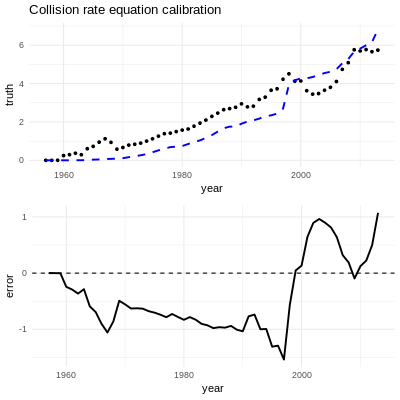
\includegraphics[width=0.5\textwidth]{../../images/risk_fit_plot.png}
	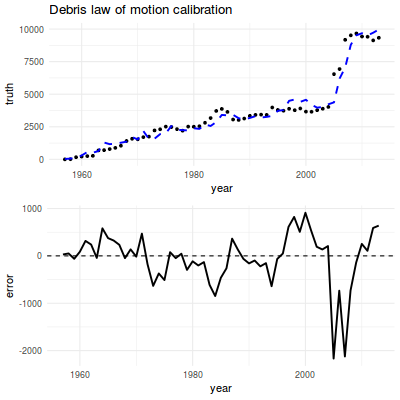
\includegraphics[width=0.5\textwidth]{../../images/debris_lom_fit_plot.png}
	\captionsetup{format=hang}
	\caption{\textit{Calibration fit.} \\
		The upper panels show fitted values (blue dashed line) against actual values (black dots). The lower panels show the residuals.
	}
	\label{debCalibration}
\end{figure}

Tables \ref{riskParms} and \ref{debParms} show the calibrated parameters:

\begin{table}[H]
	\centering
	\begin{tabular}{|l|l|l|}
		\hline
		\textit{Expected collision risk parameters:}      & \textbf{$\alpha_{SS}$} & \textbf{$\alpha_{SD}$} \\ \hline
		\textit{Parameter values:} & 1.15e-09               & 9.49e-11               \\ \hline
		\textit{Standard errors:} & 7.71e-11 & 2.2e-11 \\ \hline
	\end{tabular}
	\caption{Parameter values from estimating equation \ref{riskEstimation}.}
	\label{riskParms}
\end{table}

\begin{table}[H]
	\begin{tabular}{|l|l|l|l|l|l|l|l|}
		\hline
		\textit{Debris law of motion parameters} & \textbf{$\delta$} & \textbf{$\mu$} & \textbf{$m$} & \textbf{$\gamma_A$} & \textbf{$\beta_{SS}$} & \textbf{$\beta_{SD}$} & \textbf{$\beta_{DD}\alpha_{DD}$} \\ \hline
		\textit{Parameter values:}                           & 0.52              & 5.83           & 2.19         & 604.04              & 336.42                & 127.96                & 2.1e-05                          \\ \hline
	\end{tabular}
		\caption{Parameter values from estimating equation \ref{debLoMEstimation}. All values except $\beta_{DD}\alpha_{DD}$ are rounded to two decimal places. Standard errors are not reported due to the estimation bias in ridge regression.}
		\label{debParms}
\end{table}

These parameter values are physically plausible, with the values estimated for equation \ref{debLoMEstimation} being lower bounds\footnote{Ridge estimates are biased toward zero relative to OLS estimates. For a given penalty parameter $\lambda \geq 0$, the relationship between a ridge coefficient estimate $\hat{\beta}^{\text{ridge}}$ and the corresponding OLS estimate $\hat{\beta}^{\text{OLS}}$ is $\hat{\beta}^{\text{ridge}} = \hat{\beta}^{\text{OLS}}/(1+\lambda)$.}. For example, the value of $m$ suggests that every satellite launched creates $2.19$ pieces of debris on average, while the value of $\gamma_A$ suggests that anti-satellite missile tests create $604.04$ pieces of debris on average. While the true number is likely to be higher, the orders of magnitude between $\gamma_A$, $\beta_{SS}$, and $\beta_{SD}$ seem reasonable: firing a missile at a satellite creates the most debris due to the explosives involved, collisions between two satellites creates an intermediate amount of debris, and collisions between a satellite and  a debris fragment create the least amount of debris in part because there is the least amount of mass to be fragmented. The expected amount of debris created by debris-debris collisions is $2e-05$ fragments - a small number, but plausible considering that fragments are small and (a) unlikely to collide, and (b) have less mass to be fragmented when they do collide.

\section{Calibrating the economic model}

Our economic model draws on \cite{raorondinaWP} to determine the satellite launch rate, $X_t$, as a function of the collision risk, $\ell_{t+1}$, and the excess return on a satellite, $r_{s} - r$. In the simplest case, where all of the economic parameters are constant over time, the launch rate equates the conditional collision risk with the excess return:
\begin{equation}
\label{OAeqm}
\ell_{t+1} = \underbrace{r_s - r}_{\text{\shortstack{excess return\\on a satellite}}},
\end{equation}

where $r_s$ is the per-period rate of return on a single satellite ($\pi/F$, where $\pi$ is the per-period return generated by a satellite and $F$ is the cost of launching a satellite, inclusive of non-launch expenditures such as satellite manufacturing and ground stations) and $r$ is the risk-free interest rate.\footnote{More precisely, $r$ is the opportunity cost of funds invested in launching a satellite, and may diverge from the risk-free rate if the satellite launcher's most-preferred alternate investment is not a risk-free security. This rate is sometimes referred to as the internal rate of return (IRR).} \\

Equation \ref{OAeqm} can therefore also be used to calculate the implied IRR for satellite investments from observed data on collision risk and satellite returns. $r$ is not observed in our data. When costs, returns, and the discount rate are all time-varying, equation \ref{OAeqm} becomes
\begin{align}
\label{OAeqm2}
\ell_{t+1} &= 1+ r_{s,t+1} - (1+r_t) \frac{F_t}{F_{t+1}} \\
\implies \ell_{t+1} &= \underbrace{\left( r_{s,t+1} - r_t \frac{F_t}{F_{t+1}} \right)}_{\text{\shortstack{excess return\\on a satellite}}} + \underbrace{\left(1 - \frac{F_t}{F_{t+1}} \right)}_{\text{\shortstack{capital gains\\from open access\\and satellite launch\\cost variation}}} 
\end{align}

where $r_{s,t+1} = \pi_{t+1}/F_{t+1}$. With time-varying economic parameters, two sources of returns drive the collision risk. One is the excess return realized in $t+1$ from launching a satellite in $t$. The other is the capital gain (or loss) due to open access and the change in satellite costs. Since open access drives the value of a satellite down to the total cost of launching and operating it, $F_t$ becomes the cost of receiving $F_{t+1}$ in present value the following period, and the returns are given as percentages of $F_{t+1}$. \\

The maximum number of satellites which can be launched in a year are limited by a variety of factors, including weather, availability of rockets, and availability of launch sites. We estimate this ``launch constraint'' from the observed data for the historical period, and extrapolate it forward for the projection period. We describe this procedure in more detail in section \ref{launch_constraint} of the Appendix.

\subsection{Data}

We use data on satellite industry revenues from \citet{wienzierl2018}, and data on satellites in LEO (semi-major axis less than 2000km) from the Union of Concerned Scientists' list of active satellites \citep{UCSdata}. The economic data provide a breakdown of revenues across satellite manufacture, launch, insurance, and products and services. The satellite industry revenues data cover 2005-2015, while the active satellites data cover 1958-2017. \\

We calculate the per-period returns on owning a satellite ($\pi_t$) as the revenues generated from commercial space products and services, and the per-period costs of launching a satellite ($F_t$) as the sum of revenues from commercial infrastructure and support industries, ground stations and equipment, commercial satellite manufacturing, and commercial satellite launching. The ratio $\pi_t/F_t$ then gives a time series of the rate of return on a single satellite, as the number of satellites cancels out of the numerator and denominator. Since the numbers provided in \citet{wienzierl2018} are for the satellite industry as a whole, the ratio still needs to be adjusted to represent satellites in LEO. We do not explicitly conduct this adjustment, but let the adjustment be calculated during the estimation of equation \ref{OAeqm2}.\footnote{Another way to perform this adjustment is by calculating the yearly share of satellites in LEO and multiplying the ratio $\pi_t/F_t$ by the share in LEO. This approach is difficult to generalize to future years, and runs the risk of ``data-snooping'': since we are trying to predict the launch rate using only economic parameters (returns, costs, interest rates), incorporating the share of satellites in LEO adds physical information to the economic estimation.} \\ %We adjust for this by calculating the yearly share of satellites in LEO and multiplying the ratio by this share. \\

\subsection{Calibration procedure}

Since $r$ is unobserved, we calibrate equation \ref{OAeqm2} by estimating
\begin{equation}
\label{empiricalEqn}
\ell_t = a_{\ell 1} + a_{\ell 2} r_{st} + a_{\ell 3} \frac{F_{t-1}}{F_t} + \epsilon_{r t},
\end{equation}

using OLS on the full sample\footnote{We omit the first observation, for 2005, to construct $F_{t-1}/F_{t}$.}, where $\epsilon_{rt}$ is a mean-zero error term, $a_{\ell 2}$ is a scale parameter, and $a_{\ell 3}$ measures the gross IRR, $1+r$. The fitted values are shown against the actual values with residuals in figure \ref{econCalibration}.\footnote{While the theoretical model prescribes that $E_{t-1}[\ell_t|S_t,D_t]$ is the object being controlled by the period $t-1$ launch rate, we use the observed $\ell_t$ as a stand-in for $E_{t-1}[\ell_t|S_t,D_t]$. This is consistent with satellite launchers holding rational expectations over the future state of the orbit. While rational expectations may not be exactly true of such agents, given the planning and resources required to implement capital-intensive projects such as satellite construction and launch, we believe it to be a reasonable approximation.}

\begin{figure}[H]
	\centering
	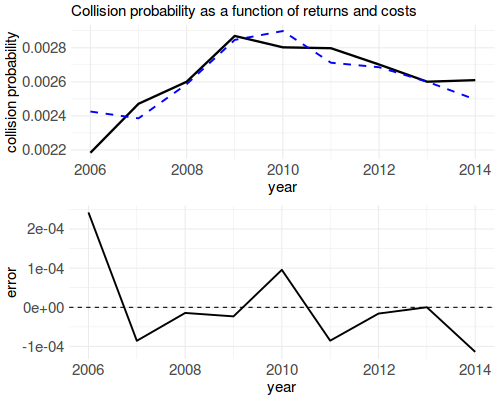
\includegraphics[width=0.5\textwidth]{../../images/risk_return_plot.png}
	\captionsetup{format=hang}
	\caption{\textit{Calibration fit.} \\
		The upper panel shows fitted values (blue dashed line) against actual values (black solid line). The lower panel shows the residuals.
	}
	\label{econCalibration}
\end{figure}

Tables \ref{econParms} shows the calibrated parameters:

\begin{table}[H]
	\centering
	\begin{tabular}{|l|l|l|l|}
		\hline
		\textit{Economic calibration parameters:}      & \textbf{$a_{\ell 1}$} & \textbf{$a_{\ell 2}$} & \textbf{$a_{\ell 3}$} \\ \hline
		\textit{Parameter values:} & 0.004               & 0.009               & - 0.0004 \\ \hline
		\textit{Standard errors:} & 0.002 & 0.002 & 0.001 \\ \hline
	\end{tabular}
	\caption{Parameter values from estimating equation \ref{OAeqm2}. All values are rounded to the first non-zero digit.}
	\label{econParms}
\end{table}

If our data perfectly measured the costs and returns of satellite ownership, and our theoretical model held exactly, we would expect $a_{\ell 1}=1$, $a_{\ell 2} = 1$, and $a_{\ell 3} < -1$. Instead, we estimate $a_{\ell 1}=0.004$, $a_{\ell 2} = 0.009$, and $a_{\ell 3} = -0.0004$. This suggests that our returns and cost series are measured with error or that our theoretical model is missing some important factors, such as constraints on the number of launches possible each period. These are discussed in \ref{attenuationFactors} in the Appendix.\\

Regardless of the factors missing from the theoretical model, we use equation \ref{empiricalEqn} to recursively calculate the sequence of launch costs implied by the combination of open access, observed launch rates, and observed satellite returns as
\begin{align}
\ell_t &= a_{\ell 1} + a_{\ell 2} r_{st} + a_{\ell 3} \frac{F_{t-1}}{F_t} + \epsilon_{r t} \nonumber \\
\implies \hat{F}_t &=	\frac{a_2 \pi_t + a_3 F_{t-1}}{\ell_t - a_1}.
\end{align}

Table \ref{launchCosts} shows the observed satellite returns ($\pi_t$), observed launch costs ($F_t$), and implied launch costs ($\hat{F}_t$).

\begin{table}[]
	\centering
	\begin{tabular}{|l|l|l|l|}
		\hline
		\textit{Year} & \multicolumn{1}{l|}{Observed return} & \multicolumn{1}{l|}{Observed cost} & \multicolumn{1}{l|}{Implied cost} \\ \hline
		\textit{2006} & 70.44                                & 161.02                             & 194.26                            \\ \hline
		\textit{2007} & 73.87                                & 185.5                              & 305.31                            \\ \hline
		\textit{2008} & 85.5                                 & 170                                & 267.32                            \\ \hline
		\textit{2009} & 93.06                                & 137.81                             & 225.56                            \\ \hline
		\textit{2010} & 101.51                               & 136.16                             & 249                               \\ \hline
		\textit{2011} & 108.84                               & 166.99                             & 264.08                            \\ \hline
		\textit{2012} & 114.55                               & 186.88                             & 295.66                            \\ \hline
		\textit{2013} & 120.25                               & 215.9                              & 301.63                            \\ \hline
		\textit{2014} & 123.18                               & 254.39                             & 299.59                            \\ \hline
	\end{tabular}
	\caption{Launch costs implied by open access and observed values. All values are given in billions of nominal US dollars per year.}
	\label{launchCosts}
\end{table}

\section{Computing satellite tax projections}

With the calibrated parameter values, we turn to computing satellite tax projections. We split this process into two stages. First, we compute open access and optimal launch policy functions in each period using the calibrated parameter values. These functions prescribe the number of satellites launched under each type of management regime for a given level of satellite and debris stocks. Then, we interpolate between solved points in the policy functions to generate launch rate predictions from the policy functions and observed orbital stocks at the start of the forecast period. We show the in-sample fit of our open access projections to establish that our approach can approximate the observed history, and then use predictions of space economy revenues and costs from \cite{MSreport} to project out the open access and optimal launch rates given those predictions. We calculate the optimal satellite tax along those time paths using the relation described in equation \ref{optTax} below:

\begin{equation}
\label{optTax}
	\tau_t = (\ell_{t+1}(\hat{S}_{t+1},\hat{D}_{t+1}) - \ell_{t+1}(S^*_{t+1},D^*_{t+1}))F_{t+1},
\end{equation}

where $\hat{S}_{t+1}$ and $\hat{D}_{t+1}$ are satellite and debris stocks in $t+1$ under open access management, and $S^*_{t+1}$ and $D^*_{t+1}$ are satellite and debris stocks in $t+1$ under optimal management. This formula is drawn from \cite{raorondinaWP}, and the optimal tax is positive as long as the planner would maintain lower collision risk than firms under open access would. Intuitively, since firms under open access set the collision risk equal to the excess return on a satellite while the planner sets the collision risk equal to the excess return of a satellite minus its marginal external cost, the difference in these collision risks gives us the marginal external cost of a satellite. By charging open access firms the marginal external cost of their satellite as a tax, their incentives are aligned with those of the planner despite the difference in legal institutions.

\subsection{Open access and optimal policy functions}

We generate two sequences of policy functions: one function for each period under consideration, and one sequence for each management regime type. We compute each sequence through backwards induction: beginning at the final period in our projection horizon, and iteratively working backwards to the initial period. This procedure implies ``perfect foresight'' planning under each management regime, i.e. that all agents under any management regime are able to perfectly forecast the sequence of returns, costs, interest rates, launch rates, and other model objects. The perfect foresight assumption is clearly unrealistic, but our purpose is not to show how uncertainty in economic parameters propagates over time. Rather, our purpose is to show how an optimal satellite tax would vary over time and the time paths of orbital aggregate stocks under different management regimes. Such assumptions are used in integrated assessment models of climate change with similar rationales, e.g. the models compared in \cite{IAMsummary}. Our work here is conceptually similar to integrated assessment modeling. \\

To compute the open access time path, we first generate a grid of satellite and debris levels, $(grid_S,grid_D)$. We generate this grid as an expanded Chebyshev grid to reduce numerical errors from interpolation, provide higher fidelity near boundaries, and economize on overall computation time. In contrast to a standard Chebyshev grid, an expanded Chebyshev grid allows for computation (rather than extrapolation) at the boundary points. The formula for the $k^{th}$ expanded Chebyshev node on an interval $[a,b]$ with $n$ points is
\[ x_k = \frac{1}{2}(a+b) + \frac{1}{2}(b-a)\sec\left( \frac{\pi}{2n} \right) \cos\left( \frac{k}{n} - \frac{1}{2n} \right) \]

We set $a=0$ and $b=25000$ for both $S$ and $D$, creating a square grid. The main issue in setting $b$ is ensuring that the time paths we solve for (described in the next section) do not run into or beyond the boundary. \\

In general, computing decentralized solutions under open access is simpler than computing the planner's solutions. This is because open access simplifies the continuation value to the cost of launching a satellite. We use \texttt{R} for all simulations, parallelizing where possible. \\

We compute optimal value functions by alternating between value function iteration and policy evaluation on a grid of the state variables $S$ and $D$. We initialize the algorithm with a guess of the value and policy functions. Algorithm \ref{vfpfi_algo} describes how we compute the optimal policy and value functions for a given grid and given value function guess $guess(S,D)$, while algorithm \ref{oa_sd_algo} describes how we compute the open access policy and value functions on the same grid. \\

We construct our initial guess of the planner's value function as the terminal value of the fleet. In the penultimate period, we assume it is not optimal to launch any satellites ($X^*_{T-1} = 0$), making the final fleet size 

\[ S_T = S_{T-1}(1-\ell_T) .\]

In the final period ($T$), the payoff of the fleet is $\pi S_T$. Our assumption that it is not optimal to launch any satellites in the penultimate period implies that the one-period returns of a satellite do not cover the cost of building and launching ($\beta \pi_T < F_{T-1}$), which we verify to hold in every period of our data. \\

To construct the implied series of $F_t$ given the observed $\pi_t$ and launch rate series', we solve equation \ref{OAeqm2} using the estimated coefficients from equation \ref{empiricalEqn}. We denote the implied launch cost as $\hat{F}_t$ and the implied rate of return on a satellite as $\hat{r}_{st}$. We use these values in solving for open access and optimal policies. \\


\begin{algorithm}[H]
	Set 
	\begin{align*} 
		W_0(S,D) &= guess(S,D), \\
		X_0 &\equiv 0
	\end{align*}
	for all $(S,D) \in (grid_S, grid_D)$
	
	Set $i=1$ and $\delta = 100$ \textit{(some large initial value)}.
	
	\While{$\delta > \epsilon $}{
		At each grid point in $(grid_S,grid_D)$, use a numerical global optimizer to obtain
		\begin{align*}
		X_i &= \text{argmax}_X \{\pi S - \hat{F} X + \beta \hat{W}_{i-1}(S',D') \}, \\
		W_i(S,D) &= \pi S - F X_i + \beta \hat{W}_{i-1}(S',D'),
		\end{align*} where $\hat{W}_{i-1}(S',D')$ is computed by linear interpolation from $W_{i-1}(S,D)$, $S' = S(1-\ell) + X_i$, $D' = D(1-\delta) + G(S,D,\ell) + mX_i$, and $\ell = \min\{a_{\ell 1} S^2 + a_{\ell 2} S D,1\}$.
		
		$\delta \leftarrow || W_i(S,D) - W_{i-1}(S,D)||_{\infty}$.\algorithmfootnote{We use $||\cdot||_{\infty}$ for the sup norm.}
		
		$\delta_{policy} \leftarrow || X^*_i - X_{i-1}||_{\infty}$
		
		\If{$\delta_{policy} < 1$ (some fixed small value),}
		{
			Evaluate the policy. Compute $W_i^T(S,D) = \sum_{t=1}^{T-1} \beta^{t-1} (\pi S_t - \hat{F} X_t^*) + W_i(S_{t+1},D_{t+1})$ by backwards induction, using the laws of motion for $S_{t+1}$ and $D_{t+1}$ and the form of $E[\ell_{t+1}|S_{t+1},D_{t+1}]$. We use progressively increasing values of $T$, beginning at $2$ and rising with $i$ to a maximum of $75$.\algorithmfootnote{This schedule for $T$ allows for error correction early on in the iterative process, while speeding up convergence later on. We found strongly diminishing marginal returns to policy evaluation beyond $75$ periods.} 
			Set $W_i(S,D) = W_i^T(S,D)$ and return to step (a). \\
		}
	i $\leftarrow$ i+1
	}
	\caption{Value function iteration with policy evaluation}\label{vfpfi_algo}
\end{algorithm}

\begin{algorithm}[H]
	Use a numerical rootfinder to find the $X_{t-1}^o$ which solves
	\[ \ell_t =  a_{\ell 1} + a_{\ell 2} \hat{r}_{st} + a_{\ell 3} \frac{\hat{F}_{t-1}}{\hat{F}_t}, \]
	where $\ell_t = \min\{ a_{\ell 1} S_t^2 + a_{\ell 2} S_t D_t, 1\}$, and $S_t = S_{t-1}(1-\ell_{t-1}) + X_{t-1}$, $D_t = D_{t-1}(1-\delta) + G(S_{t-1},D_{t-1},\ell_{t-1}) + mX_{t-1}$.
	
	Approximate $W_i^{\infty}(S,D) = \sum_{t=1}^{\infty} \beta^{t-1} (\pi S_t - \hat{F} X_t^o)$ as $W_i^T(S,D) = \sum_{t=1}^{T-1} \beta^{t-1} (\pi S_t - \hat{F} X_t^*)$ by backwards induction, using the laws of motion for $S_{t+1}$ and $D_{t+1}$ and $\ell_t = \min\{ a_{\ell 1} S_t^2 + a_{\ell 2} S_t D_t, 1\}$. We use $T=500$.
	
	\caption{Open access launch plan computation}\label{oa_sd_algo}
\end{algorithm}

\subsection{Generating time paths}

We use algorithms \ref{vfpfi_algo} and \ref{oa_sd_algo} to compute policy and value functions in each period, and run them sequentially from the final period to the first period to generate a series of policy and value functions for each period's set of economic parameters. Algorithm \ref{pfn_vfn_sequence} describes this process. \\

\begin{algorithm}[H]
	Set economic parameters to final period values.
	
	Run Algorithm \ref{vfpfi_algo} (for an optimal path) or \ref{oa_sd_algo} (for an open access path).
	
	\For{t in T-1:1} {
		Using the value function from the previous step as $W(S_{t+1},D_{t+1})$, calculate
		\[ X^* = \text{argmax}_X \{ \pi_t S - \hat{F}_t X + W(S_{t+1},D_{t+1}) \} ~~ \text{ (for an optimal path)}\]
		or
		\[ X^o : \ell_t =  a_{\ell 1} + a_{\ell 2} \hat{r}_{st} + a_{\ell 3} \frac{\hat{F}_{t-1}}{\hat{F}_t} ~~ \text{ (for an open access path)},\]
		using the laws of motion for $S_{t+1}$ and $D_{t+1}$ and $\ell_t = \min\{ a_{\ell 1} S_t^2 + a_{\ell 2} S_t D_t, 1\}$, linearly interpolating $W(S_{t+1},D_{t+1})$.
		
		If calculating an optimal path, set $W(S_t,D_t) = \pi_t S - \hat{F}_t X^* + W(S^*_{t+1},D^*_{t+1})$. If calculating an open access path, set $W(S_t,D_t) = \pi_t S - \hat{F}_t X^o + W(S^o_{t+1},D^o_{t+1})$.
	}
	\caption{Generating a perfect-foresight sequence of policy functions}\label{pfn_vfn_sequence}
\end{algorithm}

It is important to note that when obtaining the sequence of policy functions we do not do backwards induction within each economic time period prior to the final period. Instead, we hold the continuation value fixed, and iterate on the policy functions, using previous iterations as starting points. This ensures that the continuation value incorporates each period's returns and costs only once until the final period. Backwards induction on the value function in the final period treats that period's costs and returns as steady state values. \\

Once we have a sequence of policy functions for each period's economic parameters, we generate time paths by picking a starting condition $(S_0,D_0)$, computing the launch rate $X_0$ by thin-plate spline interpolation of the policy function, using the launch rate to compute the next-period state variables, and repeating the process until the terminal period. Figure \ref{projected_path_of_states} shows the simulated open access and optimal paths of launches, satellites, debris, and collision risk. Figure \ref{projected_tax_path} shows the paths of the flow of instantaneous welfare gains from open access (interpretable as the incentive to private agents to avoid self-regulation), the net present value of welfare losses from open access (the capitalized benefit to society from optimal orbit management), the price of anarchy under open access (the ratio of open access collision risk to optimal risk), and the path of an optimal satellite tax beginning in 2005.

\begin{figure}[H]
	\centering
	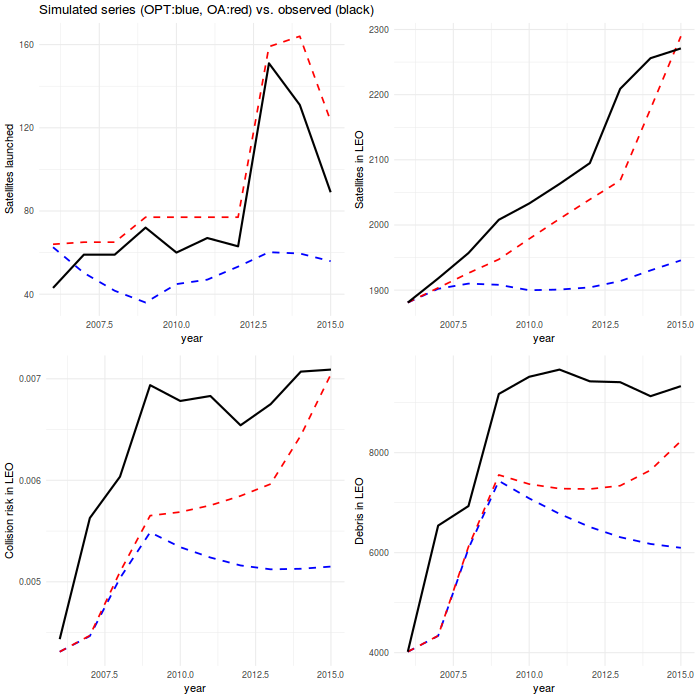
\includegraphics[width=\textwidth]{../../images/32_pt_opt_simulated_historical_series.png}
	\captionsetup{format=hang}
	\caption{\textit{Projected time paths of orbital aggregates.} \\
		The red lines show simulated open access paths. The blue lines show simulated optimal paths. The black lines show observed time paths (where data are available).
	}
	\label{projected_path_of_states}
\end{figure}

\begin{figure}[H]
	\centering
	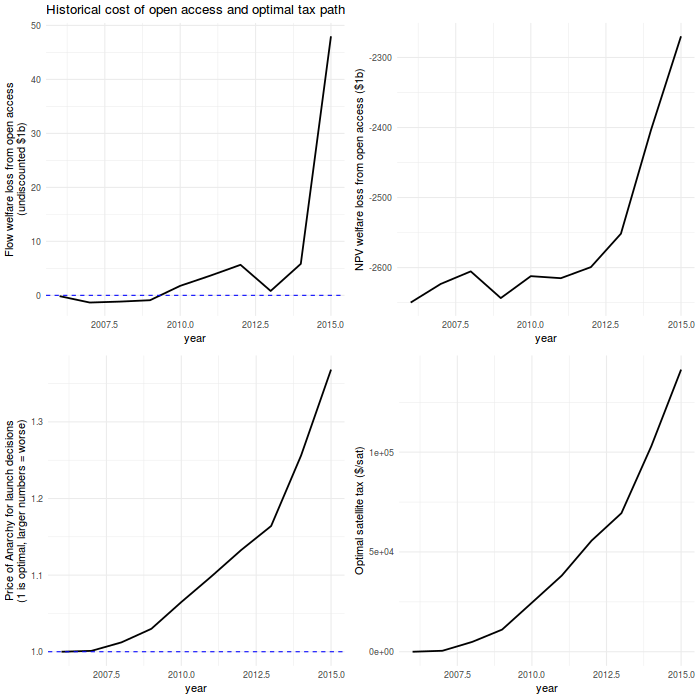
\includegraphics[width=\textwidth]{../../images/32_pt_opt_simulated_historical_cost_tax.png}
	\captionsetup{format=hang}
	\caption{\textit{Projected time paths of private gains, social losses, degree of suboptimal risk, and optimal satellite tax.} \\
		From the upper left, going clockwise: the flow of instantaneous welfare gains from open access (the incentive to private agents to avoid self-regulation), the net present value of welfare losses from open access (the capitalized benefit to society from optimal orbit management), the path of an optimal satellite tax beginning in 2005, and the price of anarchy under open access (the degree to which open access risk exceeds optimal risk).
	}
	\label{projected_tax_path}
\end{figure}

\newpage

{
	\setlength{\bibsep}{3pt}
	\setstretch{1}
	\bibliography{../database}
	\bibliographystyle{jpe}
}

\newpage

\section{Appendix}

\subsection{Sensitivity analysis of sampling procedure for estimating equation \ref{debLoMEstimation}}
\label{sensitivity}

We estimate equation \ref{debLoMEstimation} using only a quarter of the sample to avoid overfitting. To evaluate how sensitive the predictions and coefficient estimates are to our sampling procedure, we conduct a sensitivity analysis. Our procedure is straightforward. We randomly draw a quarter of the sample (15 observations) 1000 times, estimate equation \ref{debLoMEstimation} on each random sample, and plot the predictions against the observed $D_{t+1}$ in figure \ref{debSensitivityFig}. We also take the mean of the estimated coefficients and compare them against the model we selected in table \ref{debParms}. Table \ref{debSensitivityCoefs} shows the comparison.

\begin{figure}[H]
	\centering
	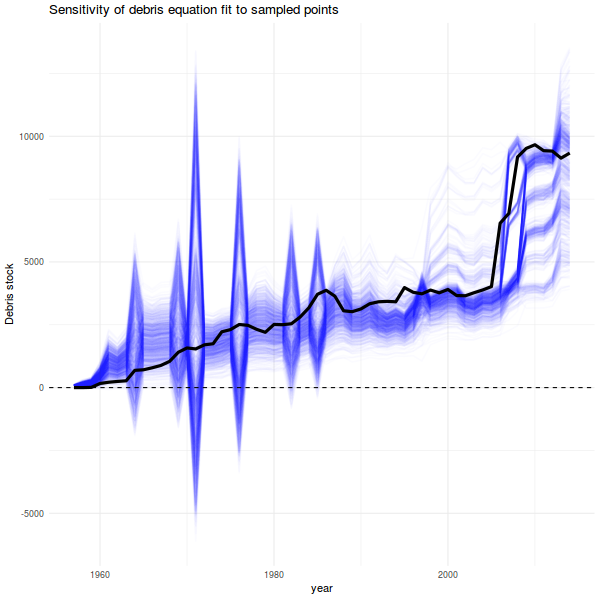
\includegraphics[width=0.7\textwidth]{../../images/debris_lom_sensitivity_plot.png}
	\captionsetup{format=hang}
	\caption{\textit{Calibration fit.} \\
		The thin blue lines show fits from random samples. The thick black line shows the actual debris time series. The large sometimes-negative spikes in the predicted series' correspond to anti-satellite missile tests, of which the 2007 FY-1C test generated the most debris.
	}
	\label{debSensitivityFig}
\end{figure}

\begin{table}[H]
	\begin{tabular}{|l|l|l|l|l|l|l|l|l|}
		\hline
		\textit{Debris law of motion parameters} & \textbf{$\delta$} & \textbf{$\mu$} & \textbf{$m$} & \textbf{$\gamma_A$} & \textbf{$\beta_{SS}$} & \textbf{$\beta_{SD}$} & \textbf{$\beta_{DD}\alpha_{DD}$} & $\lambda$ \\ \hline
		\textit{Model selected in table \ref{debParms}:}                           & 0.52              & 5.83           & 2.19         & 604.04              & 336.42                & 127.96                & 2.1e-05  &    287.21                     \\ \hline
		\textit{Mean parameter values:}                           & 0.76              & 16.19           & 2.31         & 156.57              &  487.68                & 137.94                & 1.9e-05      &  325.61                  \\ \hline
	\end{tabular}
	\caption{Parameter values from estimating equation \ref{debLoMEstimation}. All values except $\beta_{DD}\alpha_{DD}$ are rounded to two decimal places. $\lambda$ is the ridge penalty parameter, with larger values corresponding to greater shrinkage (and coefficient bias). We selected $\lambda$ by cross-validation on the training sample in all cases.}
	\label{debSensitivityCoefs}
\end{table}


\subsection{Factors which may cause coefficient attenuation}
\label{attenuationFactors}
\subsubsection{Measurement error}

Random measurement error would attenuate coefficient estimates, which may partially explain why our estimated coefficients are close to zero. Non-random measurement error is another possibility. \\

We construct the returns and costs of satellite ownership from the data described in \citet{wienzierl2018}, which aggregate revenues from all commercial satellites in orbit. Our physical model is based on data for low Earth orbit. To adjust the returns and costs to reflect only satellites in LEO, we multiply the per-period returns and cost series' by the share of satellites launched each year to LEO. If the returns to LEO satellites are lower than the returns to GEO satellites, then our attribution procedure would overstate the returns to LEO. The near-zero coefficients may therefore partially reflect systematically overstated returns to LEO in our constructed series'.

\subsubsection{Launch constraints}

Our theoretical model assumes that any firm which wants to launch a satellite can do so. If launches are limited, as they are in practice, firms will be unable to do so. This will prevent open access launching from equating the excess return on a satellite with the risk of its destruction. Firms which are able to launch will then earn rents from having a satellite while the collision risk is below the excess return. The wedge between the collision risk and excess return will reflect the value of those rents. \\

Launch limitations which allow only $\bar{X}_t$ firms to launch in $t$ are a type of ``flow control'', studied in more depth in \citet{raoJMP}. In particular, \citet{raoJMP} establishes that flow controls which restrict the quantity of launches in each period are equivalent to flow controls which impose an additional positive price $p_t$ on launching in $t$. Generalizing the flow-controlled equilibrium condition from that paper, we obtain the open access equilibrium condition for launches when costs, returns, and discount rates are all time-varying:

\begin{equation}
\label{OAfloweqmcond}
\ell_{t+1} = (1 - \frac{p_t}{F_{t+1} + p_{t+1}}) + \frac{\pi_{t+1}}{F_{t+1} + p_{t+1}} - (1+r_t)\frac{F_t}{F_{t+1} + p_{t+1}},
\end{equation}

$p_t$ can be interpreted in two ways. It may be viewed as the implied rent received by a firm which already owns a satellite in $t$ due to launches in $t$ being restricted. It may also be viewed as the implied launch tax paid by a firm which is allotted a launch slot in $t$. In either view, a binding launch constraint results in positive values of $p_t$ and $p_{t+1}$, biasing the coefficients from regression \ref{OAeqm2} downwards. %toward negative infinity ($a_{\ell 1}$) or zero ($a_{\ell 2}$ and $a_{\ell 3}$).

\subsection{Estimating the launch constraint}
\label{launch_constraint}

To prevent the model from violating the limited availability of launches, we estimate the launch constraint from the observed historical data and then project it forward. In each historical period, we calculate the maximum number of satellites which can be launched as the cumulative maximum of launch attempts (successes+failures). From the historical calculation, we project the launch constraint forward with a linear time trend and an intercept. Table \ref{lc_coefs} shows the estimated coefficients, and figure \ref{lc_time_path} shows the estimated and projected launch constraint time paths.

\begin{table}[H]
	\centering
	\begin{tabular}{|l|l|l|}
		\hline
		\textit{Launch constraint model parameters:} & Intercept & Time trend \\ \hline
		\textit{Parameter values:}                   & 30.13     & 12.5       \\ \hline
		\textit{Standard errors:}                    & 16.43     & 2.65       \\ \hline
	\end{tabular}
	\caption{Parameter values from linear model of launch constraint. All values are rounded to two decimal places. We estimate these coefficients using OLS on the historical launch constraint.}
	\label{lc_coefs}
\end{table}

\begin{figure}[H]
	\centering
	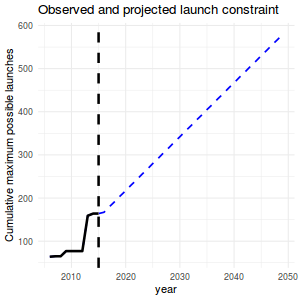
\includegraphics[width=0.7\textwidth]{../../images/linear_trend_launch_constraint.png}
	\captionsetup{format=hang}
	\caption{\textit{Launch constraint, observed and projected.} \\
		The black line shows the observed launch constraint (cumulative max of attempted launches). The blue dashed line shows a linear projection of the launch constraint.
	}
	\label{lc_time_path}
\end{figure}

\end{document}
